\begin{frame}{Activité: le plus court chemin}
  
  \begin{block}{Matériel nécessaire}
    \begin{itemize}
    \item Une planche avec des trous au hasard,
    \item autant de longs clous que de trous,
    \item une ficelle suffisamment longue et \alert{qui ne soit pas élastique},
    \item un marqueur.
    \end{itemize}
  \end{block}

  \begin{block}{Règles du jeu}
    \begin{itemize}
    \item \structure{Situation initiale :} les clous sont mis dans les trous, leurs têtes dépassent de la planche, et la ficelle est attachée à un clou par une extrémité.
    \item \structure{Comment jouer :} faire passer la ficelle \alert{une fois et une seule} par \alert{tous les clous} de la planche, puis revenir au point de départ. Le but est d'obtenir le chemin le plus court possible. À chaque fois qu'un record est battu, on fait une marque sur la ficelle pour le mémoriser.
    \end{itemize}
  \end{block}

  \begin{center}
    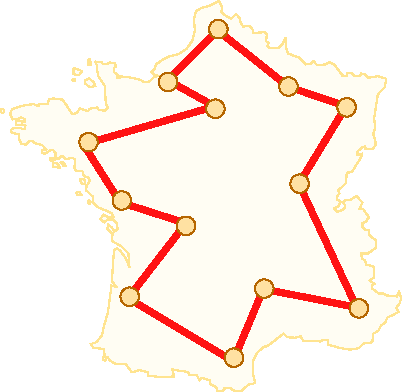
\includegraphics[width=0.3\linewidth]{img/tsp.pdf}
    \label{img:tsp}
  \end{center}

  \begin{block}{Objectif de l'activité}
    \begin{itemize}
    \item On peut construire un très grand nombre de chemins différents (pour $10$ clous, $10! = 10 \cdot 9 \cdot 8 \cdot \ldots \cdot 2 = 3628800$), et il est très difficile de trouver le meilleur chemin à coup sûr.
    \item A la place, on va chercher des méthodes (algorithmes) pour construire des chemins courts, et comparer leurs résultats.
    \end{itemize}
  \end{block}

\end{frame}

\begin{frame}{Ce qu'il faut retenir du plus court chemin : recherche de la solution optimale}
  
  \begin{itemize}
    \item Ce problème a de nombreuses applications dans la vie de tous les jours : minimiser la tournée du facteur, la longueur des pistes d'un circuit imprimé, les déplacements d'un bras robotique ... C'est un problème très étudié, plus connu sous le nom de \textbf{``problème du voyageur de commerce''}.
    \item Le problème du voyageur de commerce appartient à une catégorie de problèmes très difficiles à résoudre. Pour ces problèmes, on ne dispose pas d'algorithmes assez performants pour le résoudre quand $n$ est élevé. 
    \item Le problème du voyageur de commerce ayant fait l'objet de nombreuses études, beaucoup d'algorithmes ont été proposés pour le résoudre le plus efficacement possible.
  \end{itemize}

  \begin{block}{Trouver la solution optimale}
    
    \begin{itemize}
      \item L'approche naïve consiste à calculer la longueur de tous les chemins possibles, et comparer les résultats pour ne retenir que le plus court. 
      \item Pour $n$ villes, le nombre de chemins possible est $n!$. La performance de l'algorithme est donc $O(n!)$.
      \item Il existe cependant des algorithmes plus efficaces - par exemple, l'algorithme de Held-Karp a une performance de $O(n^{2}2^n)$. Pour illustrer la différence, comparons l'augmentation des calculs nécessaires à mesure que $n$ augmente :

      \bigskip

      \begin{center}
        \begin{tabular}{|l|cccc|}
          \hline
          nombre de sommets       & 5   & 10      & 15            & 20 \\
          \hline
          méthode naïve $O(n!)$   & 120 & 3628800 & 1307674368000 & 2432902008176640000 \\
          Held-Karp $O(n^{2}2^n)$ & 800 & 102400  & 7372800       & 419430400 \\
          \hline
        \end{tabular} 
      \end{center}

      \bigskip

      \item Ce tableau indique qu'en testant un milliard de chemins par seconde, il faudrait à la méthode naïve plus de \textbf{77 ans} pour trouver le chemin le plus court entre 20 sommets ! Dans les mêmes conditions, l'algorithme Held-Karp met moins d'\textbf{une demi seconde} pour trouver le même résultat.
    \end{itemize}
  \end{block}

  \begin{center}
    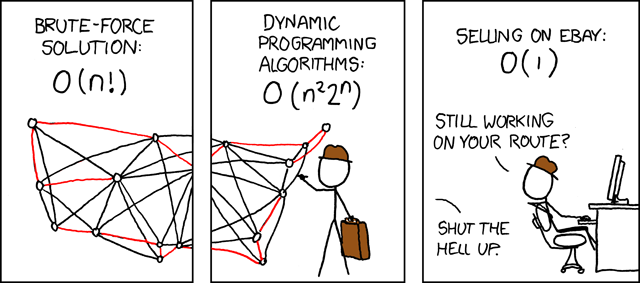
\includegraphics[width=0.7\linewidth]{img/tsp_xkcd.png}
    \label{img:tsp_xkcd}
  \end{center}

\end{frame}

\begin{frame}{Ce qu'il faut retenir du plus court chemin : recherche d'une solution approchée}

  \begin{itemize}
    \item Pour de tels problèmes, on préfère souvent trouver une solution raisonnablement bonne (solution approchée) très rapidement, plutôt que de chercher très longtemps la solution optimale. 
    \item Une \alert{heuristique} est une méthode pour fouiller intelligemment l'espace des solutions possibles à la recherche des bonnes solutions.
    \item La recherche d'heuristiques efficaces fait parti du travail des chercheurs en informatique.
  \end{itemize}
  
  \begin{block}{Les heuristiques et métaheuristiques}

    \begin{itemize}
      \item Une heuristique est spécifique au problème qu'elle traite : elle exploite certaines propriétés du problème pour orienter la recherche vers des ``régions'' succeptibles de contenir des bonnes solutions.
        % \item ajouter un exemple pour illustrer l'espace des solutions et l'exploitation d'une connaissance empirique
      \item Certaines heuristiques sont assez génériques et peuvent s'appliquer à de nombreux problèmes, moyennant quelques adaptations. On parle alors de \alert{métaheuristiques}. Les métaheuristiques sont souvent inspirées de la nature. En voici quelques exemples : 
        \begin{itemize}
          \item Le \textbf{recuit-simulé} s'inspire d'un processus utilisé en metallurgie pour minimiser l'énergie d'un matériau.
          \item Les \textbf{algorithmes génétiques} reproduisent les mécanismes de l'évolution dans le vivant : une population de solutions aléatoire est soumise à une sélection naturelle (les solutions les meilleures sont les plus adaptées) et de nouvelles solutions sont générées par croisement entre les solutions existantes et introduction de mutations aléatoires.
          \item Les \textbf{colonies de fourmis} s'inspirent du comportement des insectes sociaux : avez vous remarqué que les fourmis finissent toujours par trouver le chemin le plus court entre la fourmilière et la source de nourriture ?
        \end{itemize}
    \end{itemize}
  \end{block}

  \bigskip 

  \begin{verse}
    Un soir, alors qu'il rentre chez lui, Nasreddin perd sa bague. Un ami vient à passer par là et le voit chercher par terre sous le lampadaire. \\
    - `` Nasreddin, que t'arrive-t-il ?\\
    - Je cherche ma bague, je l'ai perdue dans l'allée un peu plus loin ...\\
    - Mais alors, pourquoi la cherches-tu ici plutôt que là bas ?\\
    - Parce qu'ici, il y a de la lumière ! ''
  \end{verse}

  % illustration, développement ?
%\end{frame}
%\begin{frame}{Ce qu'il faut retenir du plus court chemin : complexité des problèmes}

% les chercheurs classent les problèmes en fonction de la difficulté à trouver des algorithmes efficaces 
    %\item Le problème du voyageur de commerce appartient à une classe de problèmes pour lesquels il est très facile de trouver \textbf{une solution}, mais très difficile de trouver \alert{la solution optimale} en un temps raisonnable.
    %\item algos NP, NP-difficiles, NP-complets
    %\item C'est un problème qui parait bête mais qui est complexe et qui a de nombreuses applications dans la vie réelle
    %\item Exemple d'application amusante de notion de NP-complétude:  \url{http://arxiv.org/abs/1203.1895}

\end{frame}
